\section{La transformada discreta de Fourier}
\label{sec: TDF}

En esta sección vamos a dar la definición usual de 
las bases de Fourier complejas y reales, que son
bases ortonormales de $\IC^{n}$ y de $\IR^{n}$ 
\marginnote{Incluimos este capítulo de teoría clásica
por completitud de este trabajo
y para fijar la notación. 
Puede consultar referencias con
información más detallada en \TODO{cita más referencias!}}
de $\IC^{n}$
y una de $\IR^{n}$ (que llamaremos
``bases de Fourier complejas y reales''),
definidas ambas en términos de discretizaciones de
sinusoides de frecuencias enteras, y que son herramientas
clásicas para hacer lo que comúnmente se denomina
un \textbf{análisis espectral} de señales finitas.


Puesto que la definición de estas herramientas requiere
de algunas nociones del análisis complejo (en particular, de la
definición de la exponencial compleja y de las raíces $n-$ésimas
de la unidad), damos brevemente algunas definiciones y resultados
necesarios para definir las bases de Fourier.


\subsection{La exponencial compleja y raíces $n-$ésimas de la unidad}


La definición de la función exponencial compleja 
tiene diversas motivaciones
(puede consultar algunas de estas en 
\cite{marsden}). Nosotros sólo
damos la definición de esta, así como algunas propiedades
de ella que se usarán en lo que sigue.

\begin{defi}
\label{def: exponencial compleja}
Si $y \in \IR$, entonces por $exp(iy)$ denotamos al número
complejo de módulo uno y argumento $y$, es decir,
\begin{equation}
\label{eq: exponencial 1}
exp(iy) := cos(y) + i sen(y).
\end{equation}
Para todo número complejo $z = a+bi$, definimos 
$exp(z)$ como sigue:
\begin{equation}
\label{eq: exponencial 2}
exp(z) := e^{x}(cos(y) + i sen(y)).
\end{equation}
\end{defi}

\begin{prop}
\label{prop: propiedades exp compleja}
(\textbf{Algunas propiedades de la exponencial compleja}) 
Sean $z_{1}, z_{2} \in \IC$, $\omega \in \IZ$.
	\begin{itemize}
	\item $\frac{exp(z_{1})}{exp(z_{2})} = exp(z_{1} - z_{2})$
	\item $exp(z_{1} + z_{2}) = exp(z_{1}) \cdot exp(z_{2})$
	\item $(exp(z_{1}))^{\omega} = exp(\omega z)$
	\item $exp(z) = 1$ si y sólo si $z= 2K \pi i$ para algún $K \in \IZ$ 
	\item para todo $y \in \IR$, 
	\begin{equation}
	\label{eq: coseno exponenciales}
	cos(y) = \frac{exp(iy)+exp(-iy)}{2}
	\end{equation}
	y
	\begin{equation}
	\label{eq: seno exponenciales}
	sen(y) = \frac{exp(iy)-exp(-iy)}{2i}.
	\end{equation}
	\end{itemize}
\end{prop}

\begin{defi}
\label{defi: raices n esimas de la unidad}
Sea $n \in \IN$. A las $n$ raíces complejas del polinomio
$p_{n}(t)= t^{n}-1 \in \IC[t]$ 
se les denominará las \textbf{raíces $n-$ésimas de la unidad.}
\end{defi}


Las raíces $n-$ésimas de la unidad son pues los números complejos
tales que, elevados a la potencia $n$, son iguales a 1; según el 
teorema fundamental
del álgebra \ref{teo: fundamental del algebra}, sí hay números complejos
que satisfacen la definición \ref{defi: raices n esimas de la unidad}, y además
son a lo más $n$. Es fácil establecer, como hacemos a continuación, 
fórmulas explícitas para estos números, que de hecho son exactamente $n$.

\begin{prop}
Sea $n \in \IN$, $n \geq 2$. Hay exactamente $n$ raíces $n-$ésimas de la
unidad, y estas son los números complejos
 	\begin{equation}
	\label{eq3: 8ab}
	z_{n, \omega} : = exp \left( \frac{2 \pi i }{n} \omega
	\right), \hspace*{0.2cm} \textit{con} 
	\hspace*{0.2cm} \omega \in \{0, 1, \ldots, n-1 \}.
	\end{equation}
	
\end{prop}
\noindent
\textbf{Demostración.}
Por las propiedades expresadas en la proposición
\ref{prop: propiedades exp compleja}, es fácil ver que 
$z_{n,1} :=  exp \left( \frac{2 \pi i }{n} \right)$ es raíz $n-$ésima
de la unidad, pues
\[
(z_{n,1})^{n} = exp(2 \pi i ) = 1.
\]
Además, para todo $\omega \in \{ 0, \cdots , n-1 \}$, el número
\[
z_{n, \omega} : = (z_{n,1})^{\omega} = exp \left( \frac{2 \pi i }{n} \omega \right)
\]
también es es raíz $n-$ésima de la unidad, ya que

\[
(z_{n, \omega})^{n} = ((z_{n,1})^{\omega} )^{n} = 
((z_{n,1})^{n} )^{\omega} = 1^{\omega}=1. 
\]
Note ahora que los $n$ números complejos $z_{n, \omega}$ son todos 
distintos entre sí, pues si $\omega_{1}$ y $\omega_{2}$ son enteros
entre $0$ y $n-1$ tales que $z_{n, \omega_{1}} = z_{n, \omega_{2}}$,
o sea, tales que 
$exp \left( \frac{2 \pi i }{n} \omega_{1} \right) = 
exp \left( \frac{2 \pi i }{n} \omega_{1} \right)$, entonces, según el primer
punto de la proposición \ref{prop: propiedades exp compleja},
$1 = exp \left( \frac{2 \pi i }{n} (\omega_{1}-\omega_{2}) \right)$, luego, 
según el cuarto punto de esta misma proposición, $\frac{\omega_{1}-\omega_{2}}{n}$
es entero, o sea, $n$ divide a $\omega_{1}-\omega_{2}$; por el rango de 
$\omega_{1}$ y $\omega_{2}$, esto sólo ocurre si $\omega_{1}-\omega_{2}$ es
cero, o sea, si $\omega_{1}$ y $\omega_{2}$
son iguales.
\QEDB
\vspace{0.2cm}

\begin{figure}[H]
	\sidecaption{
	Para construir gráficamente a las raíces $n-$ésimas de la
	unidad, se debe dividir, a partir del punto $(0,1)$, a la
	circunferencia unitaria en $n$ partes iguales. Según esta construcción
	y la interpretación geométrica de la multiplicación compleja, es claro
	que multiplicando a $z_{n,1}$ consigo mismo se obtienen a
	todas las demás raíces $n-$ésimas.
	\label{fig: raices unidad}
	}
	\centering
	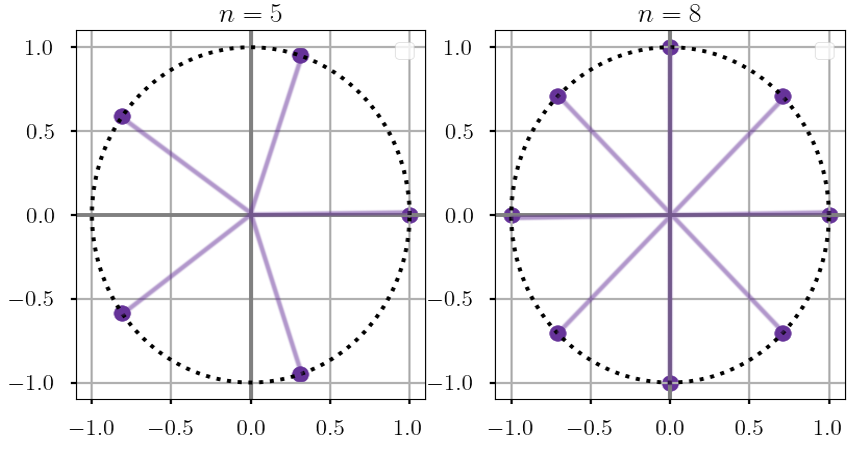
\includegraphics[scale=0.53]{raices_unidad} 
\end{figure}	


\subsection{La transformada discreta de Fourier}

Ya tenemos todo lo necesario para definir a la base
de Fourier compleja de la que hablamos al inicio.
\marginnote{El producto punto que estamos
considerando en el $\IC-$espacio
vectorial $\IC^{n}$ es el que definimos
en \eqref{eq: producto punto Cn}, y el del
$\IR-$espacio vectorial $\IR^{n}$ es el definido en 
\eqref{eq: producto punto Rn}.}

\begin{prop}
\label{prop: construccion Bn}
Sea $n \in \IN$. El conjunto

\begin{equation}
\label{eq2: 8ab}
\cali{B}_{n} : = \left\{
e_{n,\omega} = \left(
\frac{1}{\sqrt{n}} exp \left(
2 \pi i \omega \frac{m}{n}
\right)
\right)_{0 \leq m \leq n-1}
: \hspace{0.2cm} 0 \leq \omega \leq n-1
 \right\}
\end{equation}
es una base ortonormal del $\IC-$espacio
vectorial $\IC^{n}$.
\end{prop}

\noindent
\textbf{Demostración.}
Calculemos el producto punto de dos elementos
$e_{n,\omega_{1}}$ y $e_{n,\omega_{2}}$ del conjunto \eqref{eq2: 8ab};
si $\omega := \omega_{1}-\omega_{2}$,
\begin{align*}
\langle e_{n,w_{1}}, e_{n,w_{2}} \rangle = &
\frac{1}{n}
\suma{m=0}{n-1}{exp \left( 2 \pi i \frac{m}{n} \omega_{1} \right)
\cdot \overline{ exp \left( 2 \pi i \frac{m}{n} \omega_{2} \right) }} \\
= & \frac{1}{n}
\suma{m=0}{n-1}{\left( 2 \pi i \frac{m}{n} (\omega_{1}-\omega_{2}) \right)} \\
= & \frac{1}{n}\suma{m=0}{n-1}{exp\left( 2 \pi i \frac{\omega}{n} m \right)} \\
= & \frac{1}{n}\suma{m=0}{n-1}{exp\left( 2 \pi i \frac{\omega}{n}  \right)^{m}} \\
= & \frac{1}{n}\suma{m=0}{n-1}{(z_{n, \omega})^{m}};
\end{align*}

\noindent
esta última es una suma geométrica. 
\begin{itemize}
	\item Si $\omega_{1} \neq \omega_{2}$, entonces $n$ no puede dividir 
	a $\omega = \omega_{1}-\omega_{2}$ (pues, por el rango en el que se encuentran
	$\omega_{1}$ y $\omega_{2}$, $w \in [-(n-1), n-1]$, y el único múltiplo
	de $n$ en este intervalo es cero), luego, $z_{n, \omega} \neq 1$.
	En este caso se tiene entonces que 
	\[
	\langle e_{n,w_{1}}, e_{n,w_{2}} \rangle = 
	\frac{1}{n}\suma{m=0}{n-1}{(z_{n, \omega})^{m}}
	= \frac{1}{n} \cdot \frac{(z_{n, \omega})^{n}-1}{z_{n, \omega}-1}=
	\frac{1}{n} \cdot \frac{1-1}{z_{n, \omega}-1}=0.
	\]
	
	\item Si $\omega_{1} = \omega_{2}$, entonces $\omega = 0$, y
	\[
	\langle e_{n,w_{1}}, e_{n,w_{2}} \rangle = 
	\frac{1}{n}\suma{m=0}{n-1}{(z_{n, 0})^{m}}
	= \frac{1}{n}\suma{m=0}{n-1}{1} = \frac{1}{n} \cdot n = 1.
	\]
\end{itemize}

Demostramos así que los elementos de $\cali{B}_{n}$
tienen norma uno y que además
son ortogonales
dos a dos, luego, $\cali{B}_{n}$ es un subconjunto l.i. 
de $\IC^{n}$; como $\IC^{n}$ es un $\IC-$espacio vectorial de 
dimensión $n$, concluimos lo deseado.
\QEDB
\vspace{0.2cm}

Por ser \eqref{eq2: 8ab} una BON de $\IC^{n}$, siempre es
posible expresar a un vector $x = (x_{m})_{0 \leq m \leq n-1} \in \IC^{n}$
como combinación lineal de los elementos de \eqref{eq2: 8ab}
y además los coeficientes están dados por los productos punto
de $x$ y los elementos de \eqref{eq2: 8ab}
(c.f. nota \ref{nota: sobre la identidad de parseval}).

\begin{defi}
Al proceso de calcular los coeficientes de $x$
respecto a $\cali{B}_{n}$
se le conoce como el \textbf{cálculo de la 
transformada discreta de Fourier de $x$}.
\end{defi}

\marginnote{Por sus siglas en inglés, a la transformada discreta
de Fourier también se le denomina ``TDF''.}


\begin{comment}
{\Huge{\textcolor{red}{TDF}}} 

{\Huge{\textcolor{red}{Dominio: tiempo}}} 


{\Huge{\textcolor{red}{Dominio: frecuencia}}}

{\Huge{ $x = (x_{m})_{0 \leq m \leq n-1}$ }}

{\Huge{ $\langle x, e_{\omega} \rangle$, $0 \leq \omega \leq n-1 $ }}

\end{comment}


\begin{figure}[H]
\centering\captionsetup{format = hang}
	\begin{measuredfigure}
		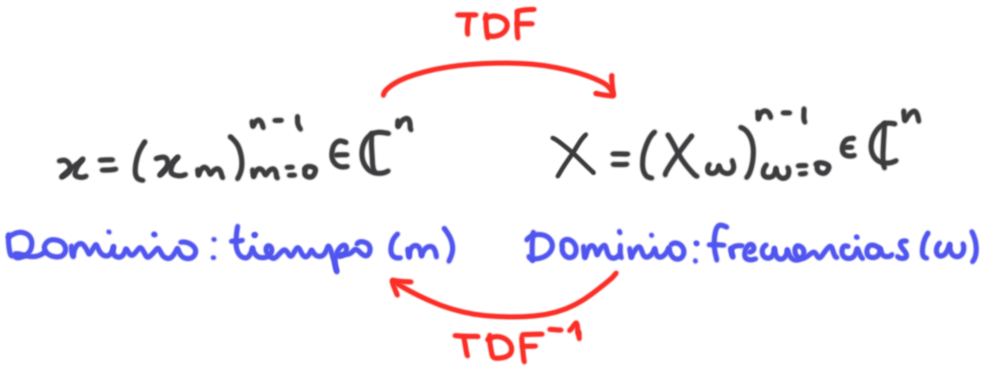
\includegraphics[scale=0.8]{tiempo_freq.png} 
		\caption{Usualmente uno representa a una señal discreta
		$x$ de dimensión $n$ con $n$ mediciones complejas; en este caso, el dominio
		de la representación es el tiempo. Pero
		también se puede representar unívocamente a $x$ con sus
		coeficientes respecto a la base de frecuencias 
		$\cali{B}_{n}$; en este caso, puesto que cada coeficiente da
		el peso que tiene la respectiva frecuencia para construir la 
		señal original $x$, decimos que el dominio de la representación
		es el de frecuencia.}
 	\end{measuredfigure}
 \end{figure}


Calcular entonces la transformada discreta de Fourier
de $x$ consiste en calcular a los productos
punto $\langle x, e_{n,\omega} \rangle $, que son

\begin{align*}
\langle x, e_{n,\omega} \rangle = & 
\frac{1}{\sqrt{n}} \suma{m=0}{n-1}{x_{m} exp \left(
2 \pi i \omega \frac{m}{n}
\right)} \\
= & 
\frac{1}{\sqrt{n}} \suma{m=0}{n-1}{x_{m} 
\left(
exp \left( \frac{2 \pi i }{n} \omega
\right) \right)^{m}} \\
= & A_{x}(z_{n, \omega}),
\end{align*}


\noindent
donde $z_{n, \omega}$ es como en \eqref{eq3: 8ab} y 
$A_{x} = A_{x}(t) \in \IC[t]$ es el polinomio de 
coeficientes complejos definido 
a partir de $x$ como sigue:

	\begin{equation}
		\label{eq4: 8ab}
		A_{x}(t) := \suma{m=0}{n-1}{\frac{x_{m}}{\sqrt{n}} t }\in \IC[t];
	\end{equation}

\noindent
así, \textbf{calcular la transformada
discreta de Fourier de $x$ es lo mismo que evaluar al polinomio 
$A_{x}$ de grado a lo más $n-1$ definido en \eqref{eq4: 8ab} en todas las raíces
$n-$ésimas de la unidad.} 


\begin{nota}
Según este último párrafo, calcular transformadas discretas
de Fourier requiere de algoritmos eficientes para evaluar
polinomios en raíces $n-$ésimas de la unidad. Usando propiedades
de las raíces $n-$ésimas de la unidad (por ejemplo,
véase el lema 30.5 de \cite{algorithms}) 
es posible usar recursión para disminuir
el tiempo de cómputo. Al algoritmo estándar usado para
esto se le conoce como la \textbf{transformada rápida de 
Fourier} (abreviado como ``FFT'' por sus siglas en inglés);
puede consultar los detalles técnicos en el capítulo
30 de \cite{algorithms}.
\end{nota}


Al usar a $\cali{B}_{n}$ como sistema de representación en
$\IC^{n}$, lo que estamos haciendo es representar a
un $x = (x_{m})_{0 \leq m \leq n-1}$ como combinación
lineal de los vectores 

\[
e_{n,\omega} = \frac{1}{\sqrt{n}} \left( cos
\left( 2 \pi \omega \frac{m}{n} \right)
+ i sen \left( 2 \pi \omega \frac{m}{n}\right) \right)_{0\leq m \leq n-1},
\hspace{0.2cm} 0 \leq \omega \leq n-1;
\]
observe que las partes reales de las
entradas de $e_{n,\omega} \in \IC^{n}$ se obtienen de tomar $n$
muestras uniformes de la función 
$c_{\omega}(t) := \frac{1}{\sqrt{n}} cos (2 \pi \omega t)$ (o sea, de la función
coseno de amplitud $\frac{1}{\sqrt{n}}$, frecuencia $\omega$ y desfase $0$)
y, similarmente,
las partes imaginarias de las entradas se obtienen muestreando
uniformemente a la función 
$s_{\omega}(t) := \frac{1}{\sqrt{n}}  sin (2 \pi \omega t)$.

\begin{figure}[H]
	\sidecaption{
	Por ejemplo, si $n=5$, para construir al vector
	$e_{3}$ de la base $\cali{B}_{n}$ se muestrean uniformemente
	cosenos y senos de frecuencia $3$ como se muestra en la figura;
	los puntos rojos representan las partes reales de las entradas
	y los azules las imaginarias.
	\label{fig: construccion Bn}
	}
	\centering
	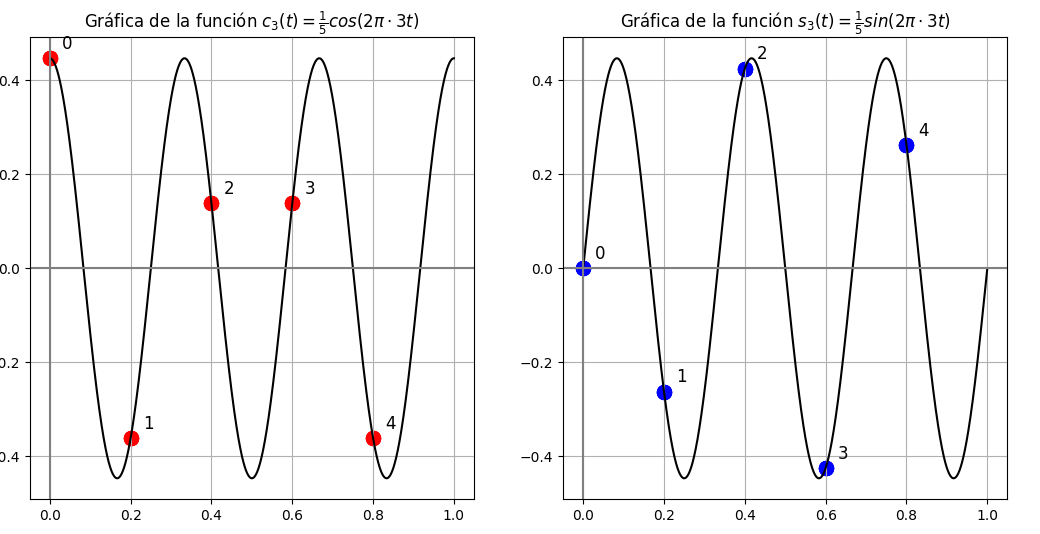
\includegraphics[scale=0.44]{construccion_Bn} 
\end{figure}	

Según esto, el vector $e_{n,\omega}$ se construye a partir
de funciones de frecuencia $\omega$; considerando esto
y el que $\cali{B}_{n}$ sea una BON de $\IC^{n}$ (luego, el
que se valga la identidad de Parseval,
c.f. nota \ref{nota: sobre la identidad de parseval}), tenemos que
la síntesis

\[
x = \suma{\omega=0}{n-1}{\langle x, e_{n,\omega} \rangle e_{n,\omega}}
\]

\noindent
es una expresión de $x$ en términos de vectores de frecuencia
$\omega$ y que los respectivos coeficientes 
$\langle x, e_{n,\omega} \rangle$ indican qué tanto 
contribuye la frecuencia $\omega$ para construir a $x$.

Es por eso que al proceso de considerar representaciones
de señales complejas finitas respecto a las bases de Fourier
se le conoce como  
\textbf{realizar un análisis espectral.}


\subsection{Versión real de la TDF}

En el caso en el que todas las entradas de un vector
$x = (x_{m})_{0 \leq m \leq n-1}$ sean reales, se puede definir
una base ortonormal de $\IR^{n}$, 
análoga a la BON $\cali{B}_{n}$ de $\IC^{n}$ construida en 
\ref{prop: construccion Bn},
a partir de muestreos uniformes
de sinusoides de frecuencias enteras.

\begin{prop}
\label{prop: base de fourier version real}
Sean $n \in \IN$ mayor a uno, $M = \lceil \frac{n}{2} \rceil$.
Definimos a los vectores de $\IR^{n}$

\[
c_{n, 0}= \left( \sqrt{\frac{1}{n}} cos
	\left(2 \pi \cdot 0 \frac{m}{n}
	\right) \right)_{m=0}^{n-1} = 
	\left( \frac{1}{\sqrt{n}}, \cdots, \frac{1}{\sqrt{n}} \right),
\]

	\begin{equation}
	\label{eq0: 10ab}
	c_{n, \omega} := \left( \sqrt{\frac{2}{n}} cos
	\left(2 \pi \omega \frac{m}{n}
	\right) \right)_{m=0}^{n-1},
	\hspace{0.2cm} 1 \leq \omega \leq M-1
	\end{equation}
	
	\begin{equation}
	\label{eq0: 4May}
	s_{n, \omega} := \left( \sqrt{\frac{2}{n}} sin
	\left(2 \pi \omega \frac{m}{n}
	\right) \right)_{m=0}^{n-1},
	\hspace{0.2cm} 1 \leq \omega \leq M-1
	\end{equation}
	
y, en el caso en que n sea par, definimos también
al vector

	\[
c_{n, M}= \left( \sqrt{\frac{1}{n}} cos
	\left(2 \pi \cdot M \frac{m}{n}
	\right) \right)_{0 \leq m \leq n-1} = 
	\left( \frac{(-1)^{m}}{\sqrt{n}} \right)_{m=0}^{n-1}.
\]

El subconjunto $\cali{F}_{n}$ de $\IR^{n}$ definido como

	\begin{itemize}
	\item $\cali{F}_{n} : = \{ c_{n,0}, c_{n,1}, s_{n,1},
	\ldots , c_{n,M-1}, s_{n,M-1}, c_{n,M} \}$ si $n$ es par
	(o sea, si $n=2M$), y como
	\item $\cali{F}_{n} : = \{ c_{n,0}, c_{n,1}, s_{n,1},
	\ldots , c_{n,M-1}, s_{n,M-1} \}$ si $n$ es impar
	(o sea, si $n=2M-1$)
	\end{itemize}
	
es una base ortonormal del $\IR-$espacio vectorial $\IR^{n}$.
\end{prop}

\noindent
\textbf{Demostración.}
Supongamos $n$ par. Si $0 \leq \omega_{1}, \omega_{2} \leq M$
son enteros, entonces
$\omega_{1} + \omega_{2}$ sólo es divisible por $n$ si ambos números
son iguales a $M$. Si suponemos a $\omega_{1}$ y $\omega_{2}$ distintos, 
entonces

\begin{align*}
\langle c_{n, \omega_{1}} , c_{n, \omega_{2}} \rangle = &
\frac{1}{n} \suma{m=0}{n-1}{cos \left(2 \pi \omega_{1} \frac{m}{n} \right) \cdot 
cos \left(2 \pi \omega_{2} \frac{m}{n} \right)} \\
= &\frac{1}{2n} \left(
cos \left(2 \pi (\omega_{1} + \omega_{2}) \frac{m}{n} \right) +
cos \left(2 \pi (\omega_{1} - \omega_{2}) \frac{m}{n} \right)
\right) \\
= & \frac{1}{4n} (
\suma{m=0}{n-1}{
(exp(2 \pi m(\omega_{1}+\omega_{2})i/n) +
exp(-2 \pi m(\omega_{1}+\omega_{2})i) } \\
&  + exp(2 \pi m(\omega_{1}-\omega_{2})i/n) +
exp(-2 \pi m(\omega_{1}-\omega_{2})i)) )\\
\textit{(suma geométrica)} = & 
\frac{exp(2 \pi i (\omega_{1}+\omega_{2}))-1}{4n (exp(2 \pi i (\omega_{1}+\omega_{2})/n)-1)} +
\frac{exp(- 2 \pi i (\omega_{1}+\omega_{2}))-1}{4n (exp(-2 \pi i (\omega_{1}+\omega_{2})/n)-1)}
\\
& + 
\frac{exp(2 \pi i (\omega_{1}-\omega_{2}))-1}{4n (exp(2 \pi i (\omega_{1}-\omega_{2})/n)-1)} +
\frac{exp(- 2 \pi i (\omega_{1}-\omega_{2}))-1}{4n (exp(-2 \pi i (\omega_{1}-\omega_{2})/n)-1)};
\\
\end{align*}

\noindent
puesto que $\omega_{1}+\omega_{2}$ y $\omega_{1}-\omega_{2}$
son ambos enteros, según la proposición 
\ref{prop: propiedades exp compleja} las exponenciales de los numeradores
de esta última expresión son todas iguales a uno, luego, 
$\langle c_{n, \omega_{1}} , c_{n, \omega_{2}} \rangle  =0$. 


Con argumentos similares se prueba 
que todos los elementos de $\cali{F}_{n}$ tienen norma uno, así como
la ortogonalidad entre dos elementos
distintos del conjunto $\cali{F}_{n}$, por lo tanto, la independencia lineal de
este conjunto, luego, el que $\cali{F}_{n}$ sea base 
(ortonormal) de $\IR^{n}$.


\QEDB
\vspace{0.2cm}



\begin{defi}
Sea $n \in \IN$, $n \geq 2$. Llamaremos a la BON
$\cali{F}_{n}$ de $\IR^{n}$ definida en \ref{prop: base de fourier version real}
la \textbf{base de Fourier real de dimensión $n$}.
\end{defi}

\begin{nota}
\label{nota: frecuencias en las bases de fourier}
Observe que $\cali{F}_{n}$, a diferencia de $\cali{B}_{n} \subseteq \IC^{n}$, 
considera frecuencias enteras no mayores a $M := \lceil \frac{n}{2} \rceil$
(cuando $n$ es par) o a $M-1$ (cuando $n$ es impar), mientras que
en $\cali{B}_{n}$ se consideran las frecuencias enteras entre $0$
y $n-1$ (inclusivo); así, si decidimos representar
a una señal $x \in \IR^{n}$ en base a $\cali{F}_{n} \subseteq \IR^{n}$
y no en base a $\cali{B}_{n} \subseteq \IC^{n}$, sintetizaremos a $x$
respecto a frecuencias enteras acotadas por $M$ o por $M-1$ 
(dependiendo de la paridad de $n$), y no respecto a frecuencias
menores a $n$.
\end{nota}

\begin{ejemplo}
\label{ej: DFT1}
Consideremos a la señal 
\begin{equation}
\label{eq2: 10ab}
x=(-0.5,-8,-5.3,15,-0.3,6,4) \in \IR^{7}.
\end{equation}

Según la construcción de $\cali{F}_{7}$ (c.f. 
proposición \ref{prop: base de fourier version real}),
una expresión de $x$ respecto a $\cali{F}_{7}$ 
es una síntesis de $x$ a partir de señales 
de frecuencias $\omega = 0,1,2,3$. En la imagen de abajo
se muestran los coeficientes de $x$ respecto a $\cali{F}_{7}$.

\begin{figure}[H]
	\sidecaption{
	Se muestran la gráfica de $x$ junto con la gráfica de los
	coeficientes de $x$ respecto a la BON $\cali{F}_{7}$. Observe 
	que, por definición, sólo un vector de $\cali{F}_{7}$ tiene frecuencia
	cero (i.e. es constante), mientras que para las otras frecuencias
	tenemos dos vectores de la misma frecuencia, uno construido a partir de un 			
	coseno y otro a partir de un seno.
	\label{fig: ejFrecuencia 1}
	}
	\centering
	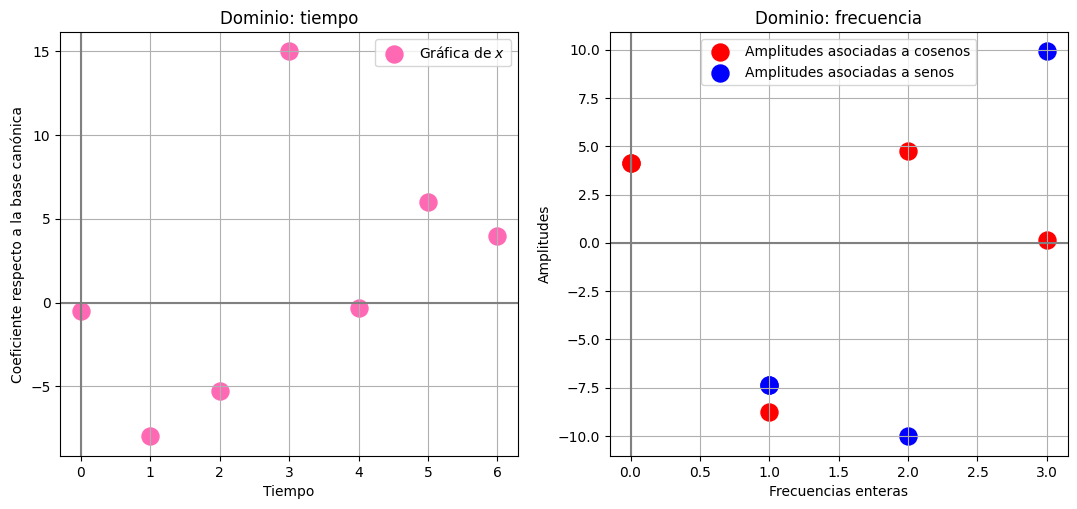
\includegraphics[scale=0.4]{ejFrecuencia_1} 
\end{figure}	

Redondeando los coeficientes, 
se tiene la siguiente descomposición de $x$;

\begin{equation}
\label{eq: analisis x TDF}
x = 4.12 c_{0} - 8.76c_{1} -7.35s_{1}+
4.77c_{2}-10s_{2}+0.14c_{3}+9.91s_{3}.
\end{equation}

\noindent
A continuación mostramos las gráficas
de los sinusoides que fueron discretizados
para obtener los vectores de frecuencia
$0,1,2$ y $3$ en los que descompusimos a $x$.

\begin{figure}[H]
	\sidecaption{
	Aporte de frecuencia $0$.
	\label{fig: ejFrecuencia 2}
	}
	\centering
	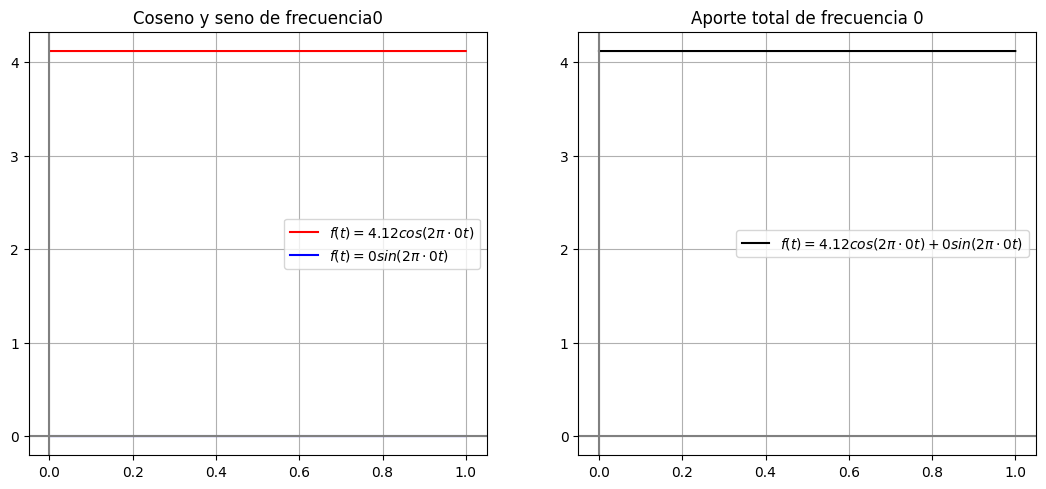
\includegraphics[scale=0.4]{ejFrecuencia_2} 
\end{figure}	

\begin{figure}[H]
	\sidecaption{
	Aporte de frecuencia $1$.
	\label{fig: ejFrecuencia 3}
	}
	\centering
	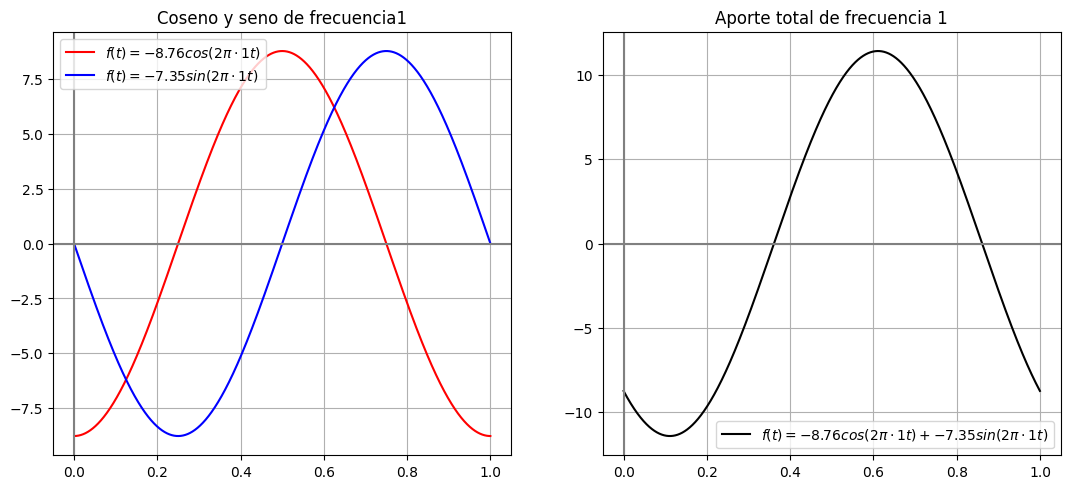
\includegraphics[scale=0.4]{ejFrecuencia_3} 
\end{figure}	

\begin{figure}[H]
	\sidecaption{
	Aporte de frecuencia $2$.
	\label{fig: ejFrecuencia 4}
	}
	\centering
	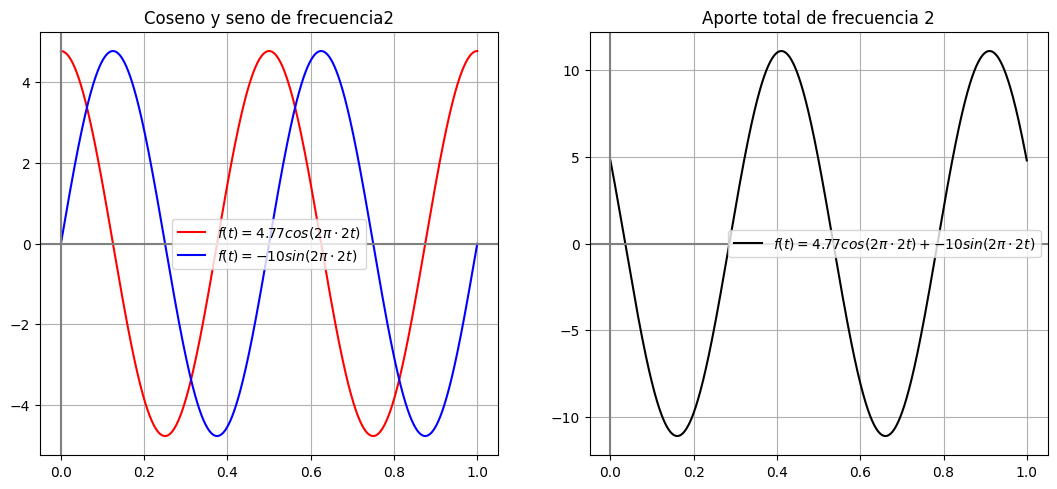
\includegraphics[scale=0.4]{ejFrecuencia_4} 
\end{figure}	


\begin{figure}[H]
	\sidecaption{
	Aporte de frecuencia $3$.
	\label{fig: ejFrecuencia 5}
	}
	\centering
	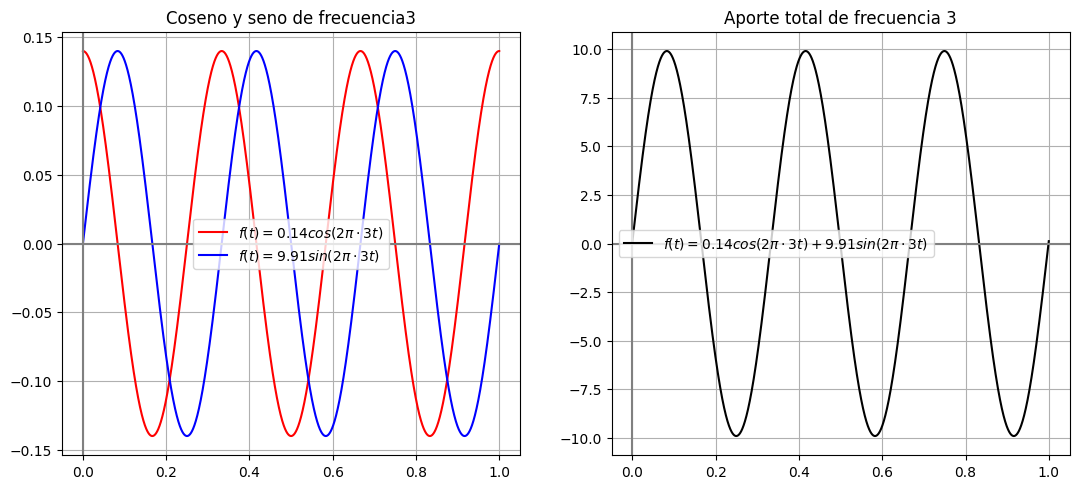
\includegraphics[scale=0.4]{ejFrecuencia_5} 
\end{figure}	

Sumando todas las gráficas de la derecha, obviamente
obtenemos una función de cosenos y senos tal que,
al muestrearla uniformemente en $[0,1]$, obtenemos
al vector $x$ \eqref{eq2: 10ab}.

\begin{figure}[H]
	\sidecaption{
	En morado se muestra la gráfica de la función suma
	de las gráficas derechas en las figuras anteriores.
	\label{fig: ejFrecuencia 6}
	}
	\centering
	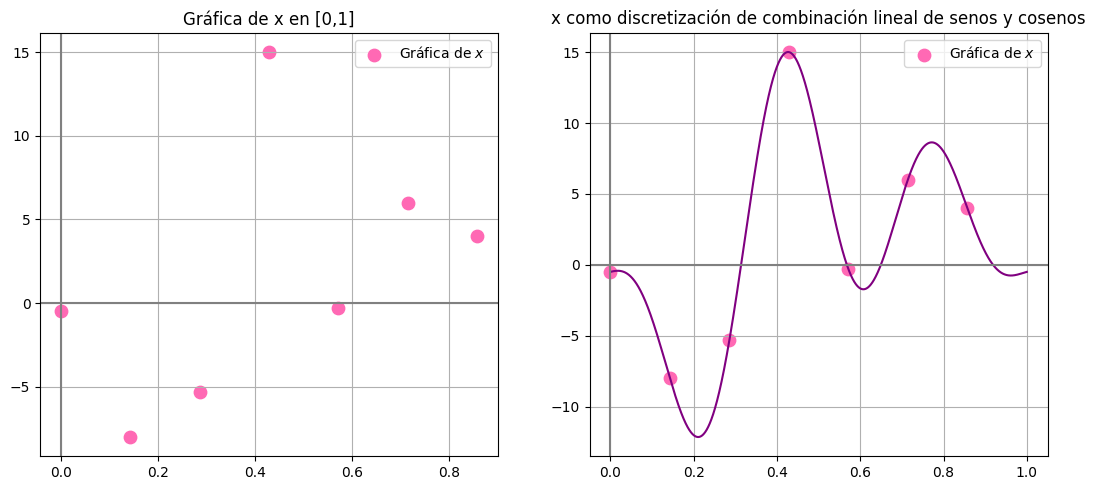
\includegraphics[scale=0.44]{ejFrecuencia_6} 
\end{figure}	
\final
\end{ejemplo}

Para terminar, digamos en concreto qué se entiende
por el espectro que resulta de usar la 
versión real de la transformada
discreta de fourier para analizar una señal finita.

En la definición 
$\cali{F}_{n}$ de la base dada en 
\ref{prop: base de fourier version real}, observe que, 
por cada frecuencia entera $\omega$ considerada,
aparecen uno o dos sinusoides (discretizados) con tal frecuencia:


\begin{table}[ht]
\sidecaption{Dimensión $n = 2M-1$ impar}
\centering
  \begin{tabular}{ l | c | c | c | c }
    \hline
    Frecuencia & $0$ & $1$ & $\ldots$ & $M-1$  \\ \hline
    Cant. sinusoides  & $1$ & $2$ & $\ldots$ & $2$ \\
    \hline
  \end{tabular}
\label{Tab: frecuencias TDF n impar}
\end{table}

\vspace{2cm}

\begin{table}[ht]
\sidecaption{Dimensión $n = 2M$ par}
\centering
  \begin{tabular}{ l | c | c | c | c | c}
    \hline
    Frecuencia & $0$ & $1$ & $\ldots$ & $M-1$ & $M$  \\ \hline
    Cant. sinusoides  & $1$ & $2$ & $\ldots$ & $2$ & $1$ \\
    \hline
  \end{tabular}
\label{Tab: frecuencias TDF n par}
\end{table}

\begin{defi}
\label{def. Dom tdf}
Sea $n \geq 2$. Llamaremos $Dom_{TDF, n}$ al conjunto de frecuencias
consideradas en la transformada discreta de Fourier para
las señales de dimensión $n$, o sea, al siguiente subconjunto de $\IR$;

\[
Dom_{TDF, n} = \{ 0 , 1, \cdots, M-1 \}
\hspace{0.2cm} \text{si } n = 2M-1
\hspace{0.2cm}
\text{es impar, }
\]
y
\[
Dom_{TDF, n} = \{ 0 , 1, \cdots, M \}
\hspace{0.2cm} \text{si } n = 2M-1
\hspace{0.2cm}
\text{es par.}
\]
\end{defi}


\noindent
Por ser $\cali{F}_{n}$ una BON de $\IR^{n}$, 
si $M = \lceil \frac{n}{2} \rceil$,
\marginnote{Recuerde que al proceso de calcular los coeficientes
de una señal respecto a una base se le conoce como 
\textbf{análisis}, mientras que el de recuperar a la señal 
via una combinación lineal con esos coeficientes 
se la llama \textbf{síntesis}.}
\[
x = \langle x , c_{n, 0} \rangle c_{n, 0}  \suma{\omega = 1}{M-1}{(
\langle x , c_{n, \omega} \rangle c_{n, \omega} + 
\langle x , s_{n, \omega} \rangle s_{n, \omega} )}
\hspace{0.2cm} \text{si n es impar}
\]
y
\[
x = \langle x , c_{n, 0} \rangle c_{n, 0} + \suma{\omega = 1}{M-1}{(
\langle x , c_{n, \omega} \rangle  c_{n, \omega} + \langle x , s_{n, \omega} \rangle
s_{n, \omega} )}
+ \langle x , c_{n, M} \rangle c_{n, M} 
\hspace{0.2cm} \text{si n es par.}
\]

Se vale además la
identidad de Parseval, luego, para toda
señal $x \in \IR^{n}$,

\begin{equation}
\label{eq0: 25Ap}
||x||^{2} = \langle x , c_{n,0} \rangle^{2}+
\suma{\omega=0}{M-1}{(\langle x , c_{n,\omega} \rangle^{2} + 
\langle x , s_{n,\omega} \rangle^{2})}
\hspace{0.2cm} \textit{si n es impar} 
\end{equation}
y
\begin{equation}
\label{eq1: 25Ap}
||x||^{2} = \langle x , c_{n,0} \rangle^{2}+
\suma{\omega=0}{M-1}{(\langle x , c_{n,\omega} \rangle^{2} + 
\langle x , s_{n,\omega} \rangle^{2})}
+ \langle x , c_{n,M} \rangle^{2}
\hspace{0.2cm} \textit{si n es par};
\end{equation}
así, los coeficientes de la forma
$\langle x , c_{n,\omega} \rangle^{2}$ y 
$\langle x , s_{n,\omega} \rangle^{2}$
dan información sobre el peso que la frecuencia
$\omega$ tiene para sintetizar a la señal $x$.

\marginnote{Según las ecuaciones \eqref{eq0: 25Ap}
y \eqref{eq1: 25Ap}, los coeficientes $\tau_{n, \omega}(x)$
permiten calibrar la presencia de la frecuencia $\omega$
(en los rangos dados por las tablas 6.1 y 6.2)
en una señal $x$.}

\begin{defi}
\label{def: taus}
Sean $n \geq 2$, $M = \lceil \frac{n}{2} \rceil $.
Definimos
	\[
	\tau_{n,0}(x) := \frac{|\langle x, c_{n,0} \rangle|}{|| x ||} ,	
	\]
	y
	\[
	\forall 
	\hspace{0.1cm}	
	1 \leq \omega \leq M-1: \hspace{0.2cm} 
	\tau_{n,\omega}(x) := 
	\frac{\sqrt{
	\langle x, c_{n,\omega} \rangle^{2}+
	\langle x, s_{n,\omega} \rangle^{2}}}{||x||}.	
	\]	
		Si $n$ es par, se define además a
	\[
	\tau_{n,M}(x) := 
	\frac{ |\langle x, c_{n,M} \rangle^{2}| }{ ||x|| }.
	\]
\end{defi}
De las ecuaciones 
\eqref{eq0: 25Ap} y 
\eqref{eq1: 25Ap} se deduce
fácilmente que, para toda $\omega$, 
$0 \leq \tau_{n, \omega}(x) \leq 1$. Puede pensar
a tales coeficientes $\tau_{n, \omega}(x)$ como la
contribución (normalizada por la norma de $x$)
de la frecuencia $\omega$ para sintetizar a $x$.


\begin{defi}
\label{def: espectro DFT}
Sean $n \geq 2$,  $x \in \IR^{n}$. Por el 
\textbf{espectro de $x$ 
obtenido a partir de la TDF} nos referiremos
a la 
función 
$\mathrm{T}_{x} : DOM_{TDF, n} \longrightarrow [0, ||x||^{2}] \subseteq \IR$
definida como
\[
\mathrm{T}_{x} (\omega) = \tau_{n, \omega}(x)
\hspace{0.2cm} \text{ para toda }
\hspace{0.2cm} \omega \in DOM_{TDF, n},
\]
donde los coeficientes $\tau_{n, \omega}(x)$
son como se definieron en \ref{def: taus}
\end{defi}

\begin{ejemplo}
A continuación se grafica el espectro
(a la derecha) obtenido
a partir de la TDF de la señal considerada en el 
ejemplo \ref{ej: DFT1}.

\begin{figure}[H]
	\sidecaption{
	Espectro de la señal $x$ dada en 
	\eqref{eq2: 10ab}. 
	\label{fig: dft_espectro_1}
	}
	\centering
	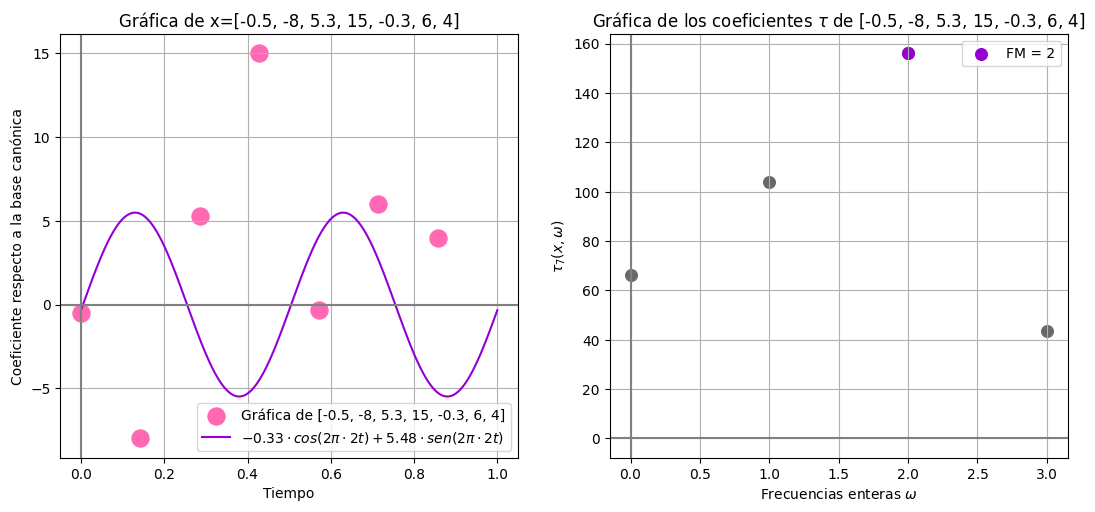
\includegraphics[scale = 0.45]{dft_espectro_1} 
\end{figure}	

Como se marca en el espectro con color morado, la frecuencia
asociada al coeficiente $\tau$ más alto es $\omega =2$; a la
izquierda, junto con la gráfica de la señal 
$x$, se dibuja el sinusoide (en versión continua)
de frecuencia $2$ que aparece en el análisis de
$x$ respecto a $\cali{F}_{7}$ dado en 
\eqref{eq: analisis x TDF}.
\final
\end{ejemplo}